\documentclass[14pt, a4paper]{article}
\usepackage[russian]{babel}
\usepackage{graphicx}
% \usepackage{tabularx}
\usepackage{layout}
\usepackage[14pt]{extsizes}
\usepackage[hidelinks]{hyperref}
\usepackage{caption}

\usepackage{listings}
\usepackage{xcolor}
\usepackage{float}
\usepackage{ulem}
\usepackage{pmboxdraw}



\setcounter{tocdepth}{4}
\setcounter{secnumdepth}{4}
\setlength{\emergencystretch}{2pt}
% \usepackage[compact]{titlesec}

\oddsidemargin = 0pt
\marginparwidth = 45pt %57
\textwidth = 467pt
\textheight = 716pt
\topmargin = 0pt %17
\footskip = 30pt %30
\headheight = 0pt %12
\headsep = 0pt %25


\definecolor{codegreen}{rgb}{0,0.6,0}
\definecolor{codegray}{rgb}{0.5,0.5,0.5}
\definecolor{codepurple}{rgb}{0.58,0,0.82}
\definecolor{backcolour}{rgb}{0.97,0.97,0.97}

\lstdefinestyle{mystyle}{
    backgroundcolor=\color{backcolour},   
    commentstyle=\color{codegreen},
    keywordstyle=\color{magenta},
    numberstyle=\tiny\color{codegray},
    stringstyle=\color{codepurple},
    basicstyle=\ttfamily\footnotesize,
    breakatwhitespace=false,         
    breaklines=true,                 
    captionpos=b,                    
    keepspaces=true,
    frame=single,                 
    % numbers=left,                    
    % numbersep=5pt,                  
    showspaces=false,                
    showstringspaces=false,
    showtabs=false,                  
    tabsize=2,
    extendedchars=\true,
    inputencoding=utf8x
}

\lstdefinelanguage{docker}{
  keywords={FROM, RUN, COPY, ADD, ENTRYPOINT, CMD,  ENV, ARG, WORKDIR, EXPOSE, LABEL, USER, VOLUME, STOPSIGNAL, ONBUILD, MAINTAINER},
  keywordstyle=\color{blue}\bfseries,
  identifierstyle=\color{black},
  sensitive=false,
  comment=[l]{\#},
  commentstyle=\color{purple}\ttfamily,
  stringstyle=\color{red}\ttfamily,
  morestring=[b]',
  morestring=[b]"
}

\lstset{
    extendedchars=\true,
    style=mystyle,
    basicstyle=\ttfamily,
    columns=fullflexible,
    keepspaces,
    literate=
    {~}{$\sim$}1%
    {┐}{\textSFiii}1%
    {└}{\textSFii}1%
    {┴}{\textSFvii}1%
    {┬}{\textSFvi}1%
    {├}{\textSFviii}{1}%
    {─}{\textSFx}1%
    {┼}{\textSFv}1%
    {│}{\textSFxi}1%
    {а}{ {\selectfont\char224} }1
    {б}{ {\selectfont\char225} }1
    {в}{ {\selectfont\char226} }1
    {г}{ {\selectfont\char227} }1
    {д}{ {\selectfont\char228} }1
    {е}{ {\selectfont\char229} }1
    {ё}{ {\"e} }1
    {ж}{ {\selectfont\char230} }1
    {з}{ {\selectfont\char231} }1
    {и}{ {\selectfont\char232} }1
    {й}{ {\selectfont\char233} }1
    {к}{ {\selectfont\char234} }1
    {л}{ {\selectfont\char235} }1
    {м}{ {\selectfont\char236} }1
    {н}{ {\selectfont\char237} }1
    {о}{ {\selectfont\char238} }1
    {п}{ {\selectfont\char239} }1
    {р}{ {\selectfont\char240} }1
    {с}{ {\selectfont\char241} }1
    {т}{ {\selectfont\char242} }1
    {у}{ {\selectfont\char243} }1
    {ф}{ {\selectfont\char244} }1
    {х}{ {\selectfont\char245} }1
    {ц}{ {\selectfont\char246} }1
    {ч}{ {\selectfont\char247} }1
    {ш}{ {\selectfont\char248} }1
    {щ}{ {\selectfont\char249} }1
    {ъ}{ {\selectfont\char250} }1
    {ы}{ {\selectfont\char251} }1
    {ь}{ {\selectfont\char252} }1
    {э}{ {\selectfont\char253} }1
    {ю}{ {\selectfont\char254} }1
    {я}{ {\selectfont\char255} }1
    {А}{ {\selectfont\char192} }1
    {Б}{ {\selectfont\char193} }1
    {В}{ {\selectfont\char194} }1
    {Г}{ {\selectfont\char195} }1
    {Д}{ {\selectfont\char196} }1
    {Е}{ {\selectfont\char197} }1
    {Ё}{ {\"E} }1
    {Ж}{ {\selectfont\char198} }1
    {З}{ {\selectfont\char199} }1
    {И}{ {\selectfont\char200} }1
    {Й}{ {\selectfont\char201} }1
    {К}{ {\selectfont\char202} }1
    {Л}{ {\selectfont\char203} }1
    {М}{ {\selectfont\char204} }1
    {Н}{ {\selectfont\char205} }1
    {О}{ {\selectfont\char206} }1
    {П}{ {\selectfont\char207} }1
    {Р}{ {\selectfont\char208} }1
    {С}{ {\selectfont\char209} }1
    {Т}{ {\selectfont\char210} }1
    {У}{ {\selectfont\char211} }1
    {Ф}{ {\selectfont\char212} }1
    {Х}{ {\selectfont\char213} }1
    {Ц}{ {\selectfont\char214} }1
    {Ч}{ {\selectfont\char215} }1
    {Ш}{ {\selectfont\char216} }1
    {Щ}{ {\selectfont\char217} }1
    {Ъ}{ {\selectfont\char218} }1
    {Ы}{ {\selectfont\char219} }1
    {Ь}{ {\selectfont\char220} }1
    {Э}{ {\selectfont\char221} }1
    {Ю}{ {\selectfont\char222} }1
    {Я}{ {\selectfont\char223} }1
}


\begin{document}

\begin{titlepage}
    \topmargin=216pt
    \newpage
    \hangindent=0.7cm
    \huge ИУ-10\\
    Системное\\
    Программное\\
    Обеспечение\\
    \textbf{Администрирование Linux\\ 
    Взаимодействие с оболочкой Bash}

    \vspace{10cm}

    \begin{center}
        \small\textit{Москва, 2022}
    \end{center}
\end{titlepage}
\section*{На этом уроке}
\begin{enumerate}
    \item Узнаем, как подключиться к ОС, используя протокол удалённого управления SSH.
    \item Изучим, как работает навигация по файловой системе
    \item Познакомимся с утилитами работы с папками
    \item Познакомимся с утилитами работы с файлами
    \item Научимся искать информацию в документации с man
\end{enumerate}
\tableofcontents
\newpage



\section*{Знакомство с Bash}
\addcontentsline{toc}{section}{Знакомство с Bash}


Как мы узнали на первом уроке Linux может быть использован как в десктопной версии, так и в
серверной. В десктопной версии используется графический интерфейс, и вы можете работать в
окружении рабочего стола, схожего с тем, что вы используете в Windows. Так как основное
достоинство Linux — применение в серверном администрировании, администраторы для работы
используют интерфейс командной строки (Command Line Interface - CLI) или консоль, только в нем
доступен весь функционал Linux.

Консоль позволяет нам вводить текстовые команды, получать ответ системы на них в
текстовом виде и таким образом управлять операционной системой. \textbf{Важно!} \textit{\uline{Оболочка Bash - это
интерпретатор команд, который используется по умолчанию, то есть любая вводимая команда
будет обрабатываться Bash. Оболочка предоставляет набор полезных функций, которые мы
изучим на уроке.}}

После загрузки ОС нам становится доступно семь терминалов, переключаться между
которыми можно, используя комбинацию клавиш.

\begin{enumerate}
    \item В случае с физической машиной: \textbf{Ctrl + Alt + F(1–7)}, где клавиши F1–F7 — номера
    виртуальных терминалов
    \item В случае с виртуальной машиной (под VirtualBox) переключение между терминалами будет
    осуществляться при помощи комбинации \linebreak \textbf{host\_key + F(1–7)}, где host\_key в большинстве
    случаев — клавиша правый Ctrl.
\end{enumerate}

Для последующей работы будем использовать подключение к серверу через протокол SSH.
Для этого нам понадобится установить на свой компьютер клиент SSH. Самый распространенный
клиент для Windows — \href{https://www.putty.org/}{PuTTY}, в последних версиях ОС Windows существует встроенный клиент. Если
вы работаете из-под Linux или macOS, то для подключения к удалённому серверу можно
использовать предустановленный в системе клиент.

\begin{enumerate}
    \item \textbf{Подключение к серверу, используя PuTTY}. Запускаем программу. В поле Host Name (or IP
    address) вводим IP-адрес нашей виртуальной машины или сервера. Далее нажимаем кнопку
    Open, вводим логин и пароль. \textbf{Важно:} \textit{\uline{при вводе пароля символы не отображаются.}}
    \begin{figure}[H]%current location
        \centering
        \scalebox{1}{
\includegraphics[width=0.8\textwidth]{imgs/1.0.png}}
        \label{1.0}
    \end{figure}
    \item Подключение к серверу, используя terminal/iTerm. Запускаем программу и в окне вводим
    команду \colorbox{backcolour}{SSH your\_user@ip\_server}, далее вводим пароль и получаем приглашение в
    командную строку.
\end{enumerate}

\textbf{Примечание.} \textit{\uline{Найти IP адрес сервера можно с помощью команды \textbf{ip address show}, как показано
ниже на рисунке. Команду требуется ввести после логина через терминал VirtualBox.}}

\begin{figure}[H]%current location
    \centering
    \scalebox{1}{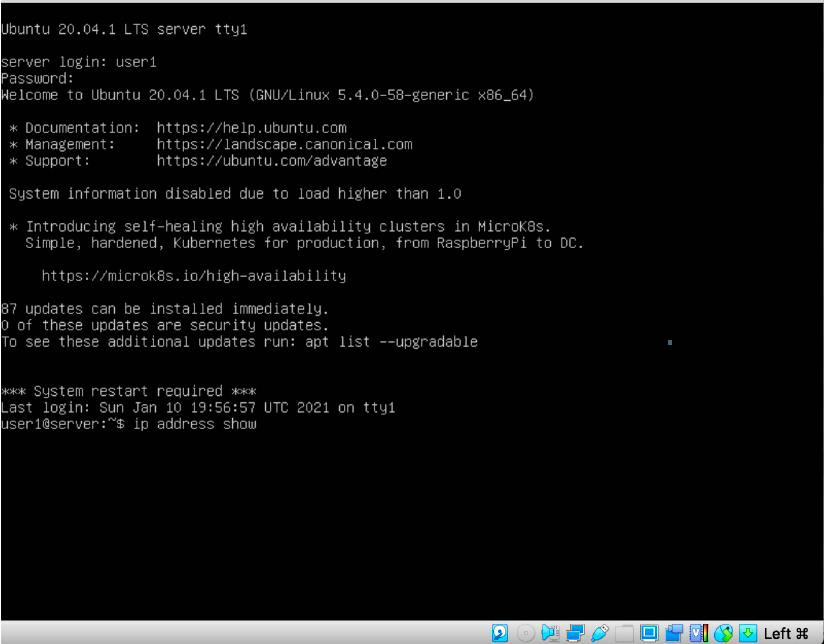
\includegraphics[width=0.9\textwidth]{imgs/1.1.png}}
    \scalebox{1}{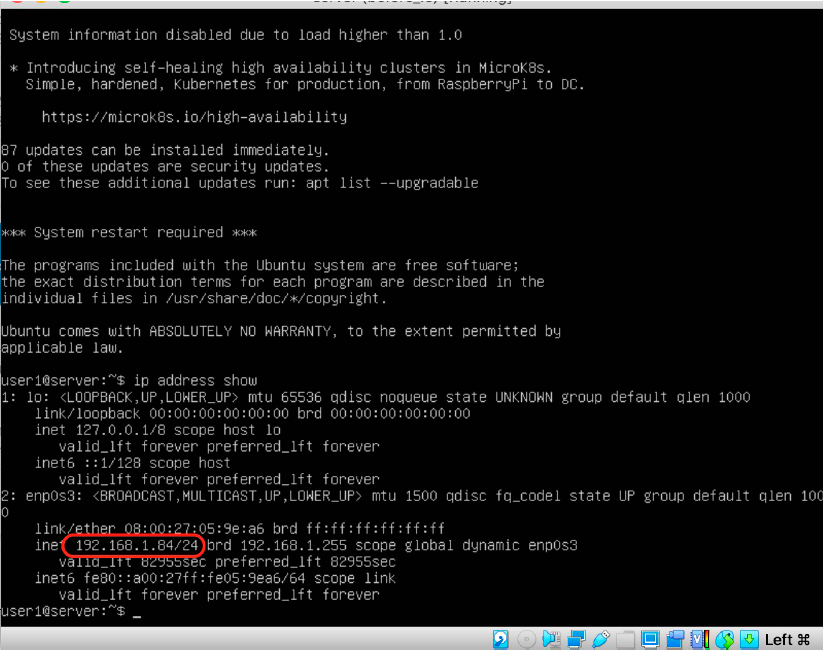
\includegraphics[width=0.9\textwidth]{imgs/1.2.png}}
    \label{1.0}
\end{figure}


\subsection*{Навигация по файловой системе и основные операции с
файлами и каталогами}
\addcontentsline{toc}{subsection}{Навигация по файловой системе и основные операции с
файлами и каталогами}

Хранение файлов в Linux организовано в виде древовидной структуры. В ней есть корневой
каталог, от которого «растут» все остальные каталоги и файлы. Корневой каталог носит название «/»
(root), при этом важно не путать его с домашним каталогом суперпользователя /root. Утилита \colorbox{backcolour}{tree}
выведет на экран иерархию на экран.

\begin{figure}[h]%current location
    \centering
    \scalebox{1}{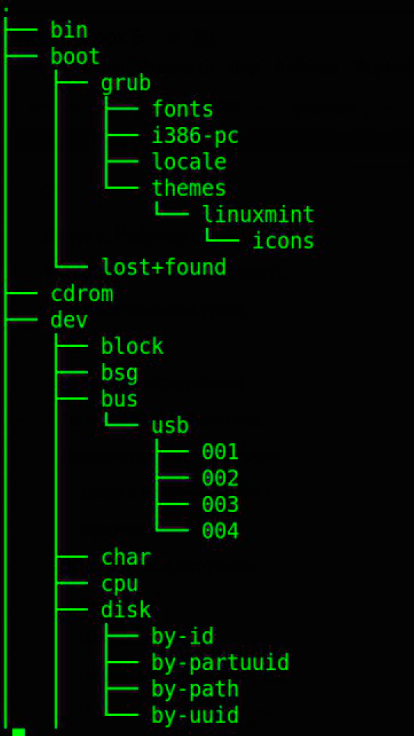
\includegraphics[width=0.6\textwidth]{imgs/1.3.png}}
    \label{1.0}
\end{figure}

В оконном интерфейсе Windows навигация по системе интуитивно понятна, так как
используются визуальные образы и нажатия клавиш мыши. В интерфейсе командной строки
подобное представление отсутствует, поэтому для успешной навигации по файловой системе в
первую очередь необходимо разобраться в понятии \href{https://ru.wikipedia.org/wiki/%D0%9F%D1%83%D1%82%D1%8C_%D0%BA_%D1%84%D0%B0%D0%B9%D0%BB%D1%83}{пути до файла или каталога}.

Путь до файла - это набор символов, показывающий расположение файла или каталога
(папки) в файловой системе. По сути путь указывает нам, в какой точке дерева в данный момент
мы находимся. Путь может быть полным (абсолютным) — это путь, который указывает на одно и то
же место в файловой системе, вне зависимости от текущего рабочего каталога. \textbf{Примечание!} \textit{\uline{Полный
путь всегда начинается с корня - “/”(слэш), например /usr/local/bin/}}. Путь может быть также
относительным — это путь по отношению к текущему рабочему каталогу пользователя (то есть по
отношению к директории в которой пользователь сейчас находится). В отличие от абсолютного пути,
относительный меняется, если мы меняем нашу текущую директорию. \textbf{Примечание!}
\textit{\uline{Относительный путь никогда не начинается с корня - “/”(слэш), например local/bin/}}.

Команда \colorbox{backcolour}{pwd — print working directory} (показать рабочий каталог) — это первая
команда, с которой мы познакомимся. Она покажет текущий каталог (каталог, в котором мы сейчас
находимся), при этом покажет полный путь. Команда необходима, чтобы понять, в каком месте дерева
файловой системы мы находимся.

\begin{lstlisting}
user@server:~$ pwd
/home/user
user@server:~$
\end{lstlisting}

Перемещение между каталогами осуществляется при помощи команды \textbf{cd — change
directory}. Данная команда позволит нам сменить текущую директорию, используя полный или
относительный путь. Например:

\begin{itemize}
    \item используем полный путь: \colorbox{backcolour}{cd /var/log};
\begin{lstlisting}
user@server:~$ pwd
/home/user
user@server:/var/log$ cd /var/log/
user@server:/var/log$ pwd
/var/log
\end{lstlisting}
    \item используем относительный путь: \colorbox{backcolour}{cd journal/};
\begin{lstlisting}
user@server:/var/log$ cd journal/
user@server:/var/log/journal$ pwd
/var/log/journal
\end{lstlisting}
    \item для перехода на уровень выше можно использовать \colorbox{backcolour}{cd ..}
\begin{lstlisting}
user@server:/var/log/journal$ cd ..
user@server:/var/log$ pwd
/var/log
\end{lstlisting}
    \item быстро вернуться в домашний каталог: \colorbox{backcolour}{cd $\sim$} или просто \colorbox{backcolour}{cd}
\begin{lstlisting}
user@server:/var/log$ cd
user@server:~$ pwd
/home/user1
user@server:~$
\end{lstlisting}
    \item Переход в предыдущую директорию: \colorbox{backcolour}{cd -}
    
\begin{lstlisting}
user@server:~$cd -
user@server:/var/log$
\end{lstlisting}
\end{itemize}



\subsection*{Полезные функции Bash}
\addcontentsline{toc}{subsection}{Полезные функции Bash}

При работе в командном интерпретаторе bash есть несколько комбинаций клавиш,
позволяющих существенно облегчить работу. Например, в параметрах команд можно не набирать
имена существующих файлов или каталогов целиком, достаточно набрать их начало и нажать
клавишу табуляции.

\begin{lstlisting}
user@server:~$ cd f<TAB>
\end{lstlisting}

Дальше bash выполнит поиск среди файлов, начинающихся на f, и в случае однозначного
совпадения имя будет сразу дополнено:

\begin{lstlisting}
user@server:~$ cd files/
\end{lstlisting}

Если найденных вариантов несколько, они все будут показаны:

\begin{lstlisting}
user@server:~/files$ cd 20<TAB>
2000/ 2002/ 2004/ 2006/ 2008/ 2010/ 2012/ 2014/
2001/ 2003/ 2005/ 2007/ 2009/ 2011/ 2013/
\end{lstlisting}

Можно продолжить набор, сократив количество вариантов:
\begin{lstlisting}
user@server:~/files$ cd 201<TAB>
2010/ 2011/ 2012/ 2013/ 2014/
\end{lstlisting}

Аналогично работает автодополнение по именам команд:

\begin{lstlisting}
user@server:~/files$ ma<TAB

mailmail3    man          manifes      man-recode
    
make-bcache  mandb        manpat       mapfil       mawk    
\end{lstlisting}

Кроме автодополнения существует возможность повторять ранее набранные команды с
помощью стрелочек вверх-вниз на клавиатуре. Это называется историей или стеком команд. Команда
history выведет на экран все ранее вводимые команды и с помощью комбинации !<номер> команду
можно повторить.

\begin{lstlisting}
user@server:~$ history
1  cd /var/log/
2  pwd
3  cd /var/log/
4  pwd
5  cd journal/
6  pwd
7  cd
8  pwd
9  cd /var/log/
10  ls
11 clear
user1@server:~$ !3
cd /var/log/
user@server:/var/log$
\end{lstlisting}

Можно выполнять поиск по истории команд с помощью комбинации Ctrl-R (поиск
назад).Введите строку поиска и если в истории команд была команда с такой подстрокой, она
будет найдена и предложена к выполнению.

\begin{lstlisting}
(reverse-i-search)`cd': cd /var/log/
\end{lstlisting}

Используйте Enter для немедленного выполнения команды или <ESC>, чтобы найденную
команду редактировать.

Кроме того, существуют команды для быстрого перемещения по командной строке и
быстрого удаления текста:

\begin{itemize}
    \item Ctrl-A — в начало строки.
    \item Ctrl-E — в конец строки.
    \item Alt-F — на слово вперед.
    \item Alt-B — на слово назад.
    \item Ctrl-U — удалить в строке все символы от текущей позиции до начала строки.
    \item Ctrl-K — удалить в строке все символы от текущей позиции до конца строки.
\end{itemize}
\textbf{Примечание!} \textit{\uline{Заглавные буквы показаны только для наглядности, комби\-нации работают со
строчными символами.}}




\section*{Взаимодействие с файлами и каталогами}
\addcontentsline{toc}{section}{Взаимодействие с файлами и каталогами}

\subsection*{Просмотр и создание}
\addcontentsline{toc}{subsection}{Просмотр и создание}

Просмотреть содержимое каталога нам поможет команда \textbf{ls <путь к каталогу>}. Если путь к
каталогу не указан, то будет показано содержимое папки, в которой находится пользователь в данный
момент. У команды есть ряд полезных ключей (параметров):

\begin{enumerate}
    \item \colorbox{backcolour}{ls -l} покажет подробный список содержимого, сюда будут включены дата изменения,
    владелец и группа владельца, права и другие свойства файлов или каталогов в директории.
    \item \colorbox{backcolour}{ls -a} покажет скрытые файлы и каталоги. В Unix-подобных системах такие файлы и каталоги
    начинаются с точки. Этот параметр очень часто используют в сочетании с параметром \textbf{-l},
    например \colorbox{backcolour}{ls -al /home/user}.
\end{enumerate}
\begin{lstlisting}
user@server:~$ ls -al
total 24
drwxr-xr-x 2 user user 4096 Dec 30 14:55 .

drwxr-xr-x 6 root root 4096 Dec 14 18:04 ..

-rw------- 1 user user 153 Dec 24 17:11 .bash_history

-rw-r--r-- 1 user user 220 Feb 25 2020 .bash_logout

-rw-r--r-- 1 user user 3771 Feb 25 2020 .bashrc
-rw-rw-r-- 1 user user    0 Dec 30 14:55

-rw-rw-r-- 1 user user    0 Dec 30

-rw-r--r-- 1 user user 807 Feb 25 2020 .profile

-rw-r--r-- 1 user user    0 Dec 13 18:42 .sudo_as_admin_successful
\end{lstlisting}

Для создания файлов в ОС Linux есть несколько способов:

\begin{enumerate}
    \item Используя утилиту \textbf{touch} — она создаст пустой файл.
    \item Используя перенаправление потока вывода, например, с помощью утилит \textbf{cat} или \textbf{echo}
    (рассмотрим их на следующем уроке).
    \item Используя текстовый редактор.
\end{enumerate}

Создание каталогов — команда \textbf{mkdir} (в некоторых дистрибутивах \textbf{md}, make directory).
Например, \colorbox{backcolour}{mkdir /home/user/dir1} создаст каталог с именем dir1 в домашнем каталоге
пользователя user.

Бывают случаи, когда нам необходимо создать каталог и вложенные подкаталоги, для
решения этой задачи используют параметр \textbf{-p (parents)}, например, \colorbox{backcolour}{mkdir -p
/home/user/dir1/dir2/} создаст в домашнем каталоге пользователя user каталог dir1 и вложенный
подкаталог dir2.

\begin{lstlisting}
user@server:~$ mkdir /home/user/dir1/dir2/
mkdir: cannot create directory ‘/home/user/dir1/dir2/’: No such file or
directory
user@server:~$ mkdir -p /home/user/dir1/dir2/
user@server:~$ tree
.
├── dir1
│   └── dir2
├── file1
└── file2
\end{lstlisting}

\subsection*{Действия с существующими объектами}
\addcontentsline{toc}{subsection}{Действия с существующими объектами}

Копирование файлов или каталогов — команда \textbf{cp (copy): cp file1 file2}. При операции
копирования можно использовать как полный, так и относительный путь. Например:

\begin{itemize}
    \item \colorbox{backcolour}{cp /usr/local/etc/file /tmp/} скопирует файл с именем file из каталога /usr/local/etc/ в
    каталог /tmp, сохранив название файла.
    \item \colorbox{backcolour}{cp /usr/local/etc/file /tmp/file1} скопирует файл с именем file из каталога
    /usr/local/etc/ в каталог /tmp, изменив имя файла на file1.
    \item \colorbox{backcolour}{cp /usr/local/etc/file .} копирует файл из каталога /usr/local/etc/ в текущий каталог.
    \item \colorbox{backcolour}{cp file file1} создаст копию файла в текущем каталоге.
    \item Копирование директорий происходит немного иначе, поскольку может содержать
    поддиректории, поэтому необходимо использовать параметр \textbf{-r (рекурсивно)}, например, \colorbox{backcolour}{cp
    -r /dir1 .} скопирует каталог /dir1 в текущую директорию.
\end{itemize}

\begin{lstlisting}
user1@server:~$ cp dir1/ copy_dir1
cp: -r not specified; omitting directory 'dir1/' user1@server:~$ cp -r  dir1/ copy_dir1 
user1@server:~$ tree
.
├── copy_dir1
│   └── dir2
├── dir1
│   └── dir2
├── file1
└── file2
\end{lstlisting}

Перемещение файлов или каталогов — команда \textbf{mv (move)}. \linebreak \colorbox{backcolour}{mv /home/user/file
/home/user1/file} переместит файл из каталога \linebreak /home/user в каталог /home/user1. Команда \textbf{mv},
применённая к файлу или каталогу в текущей директории, переименует файл или каталог. Например:
\colorbox{backcolour}{mv file1 file2, mv dir1 dir2}. \textbf{Примечание!} \textit{\uline{Относительно каталогов операция mv не
требует параметра -r, поскольку никак не воздействует на поддиректории}}.

Удаление файлов или каталогов — команда \textbf{rm (remove)}. Например, \colorbox{backcolour}{rm file1} удалит файл.
Для удаления каталогов необходимо использовать параметр \textbf{-rf} (recursive, forced) — удалить со всем
содержимым, не спрашивая подтверждения.

\textbf{Внимание!} \textit{\uline{Операция удаления — необратимое действие. \
\linebreak Debian-подобные дистрибутивыне спрашивают подтверждения
\linebreak действия. Ошибочное удаление файлов или каталогов может привести 
к не\-ра\-бо\-то\-способности системы}}.




\subsection*{Функция globbing в Bash}
\addcontentsline{toc}{subsection}{Функция globbing в Bash}

globbing - это функция оболочки, которая помогает в сопоставлении имен файлов. Его не следует
путать с регулярными выражениями, тема, о которой мы поговорим позже, и которая поможет найти
текстовые шаблоны.

Давайте разберем несколько примеров, как пользоваться globbing.


\begin{lstlisting}
kglushen@server:~$ ls -l /etc/host*
-rw-r--r-- 1 root root 92 Dec 5 2019 /etc/host.conf

-rw-r--r-- 1 root root   7 Jan 28 14:22 /etc/hostname

-rw-r--r-- 1 root root 221 Jan 28 14:22 /etc/hosts

-rw-r--r-- 1 root root 411 Jan 28 14:23 /etc/hosts.allow
-rw-r--r-- 1 root root 711 Jan 28 14:23 /etc/hosts.deny
\end{lstlisting}

Можно видеть, что были показаны все файлы, имена которых начинаются с host, за которыми следует
что угодно (символ *). С помощью “?” шаблон будет подставлять один любой символ, а в квадратных
скобках задается перечень ожидаемых символов, или символов, которые нужно исключить (для этого
применяется восклицательный знак).

\begin{lstlisting}
kglushen@server:~$ touch cat kglushen@server:~$ touch hat kglushen@server:~$ touch rat 
kglushen@server:~$ touch canat
kglushen@server:~$ ls -l ?at
-rw-rw-r-- 1 kglushen kglushen 0 Jan 30 13:24 cat
-rw-rw-r-- 1 kglushen kglushen 0 Jan 30 13:24 hat
-rw-rw-r-- 1 kglushen kglushen 0 Jan 30 13:24 rat 

kglushen@server:~$ ls -l [ch]at
-rw-rw-r-- 1 kglushen kglushen 0 Jan 30 13:24 cat
-rw-rw-r-- 1 kglushen kglushen 0 Jan 30 13:24 hat kglushen@server:~$ ls -l [!ch]at
-rw-rw-r-- 1 kglushen kglushen 0 Jan 30 13:24 rat
\end{lstlisting}

С помощью globbing в шаблоне можно указывать диапазон чисел.

\begin{lstlisting}
kglushen@server:~$ touch {1..5}_file
kglushen@server:~$ ls -l *_file
-rw-rw-r-- 1 kglushen kglushen 0 Jan 30 13:35 1_file
-rw-rw-r-- 1 kglushen kglushen 0 Jan 30 13:35 2_file
-rw-rw-r-- 1 kglushen kglushen 0 Jan 30 13:35 3_file
-rw-rw-r-- 1 kglushen kglushen 0 Jan 30 13:35 4_file
-rw-rw-r-- 1 kglushen kglushen 0 Jan 30 13:35 5_file
kglushen@server:~$ ls -l [1-3]_file
-rw-rw-r-- 1 kglushen kglushen 0 Jan 30 13:35 1_file
-rw-rw-r-- 1 kglushen kglushen 0 Jan 30 13:35 2_file
-rw-rw-r-- 1 kglushen kglushen 0 Jan 30 13:35 3_file
\end{lstlisting}


\subsection*{Архиваторы и компрессоры в Linux}
\addcontentsline{toc}{subsection}{Архиваторы и компрессоры в Linux}

В Windows вы наверняка использовали программы-архиваторы (rar и zip), которые позволяют
упаковать каталог c файлами в один сжатый архивный файл. В Linux тоже есть версии этих
архиваторов, которыми можно распаковать архивы, созданные пользователями Windows. Также есть
графические программы-оболочки, облегчающие пользователям работу с архивами. Сейчас мы
поговорим о других программах из мира Linux, которые появились задолго до своих
Windows-собратьев. Чем же они уникальны?

Во-первых, есть различие в терминах. Архиваторами в Linux и Windows называют программы,
немного отличающиеся по назначению. В Linux архиваторы выполняют следующие задачи:

\begin{lstlisting}
    \item создавать архивы как объединения заданных файлов в виде одного
    \item добавлять в архив или извлекать из него отдельные файлы или группы файлов.
\end{lstlisting}

В Windows архиваторы делают то же что в Linux, плюс дополнительно занимаются сжатием
архивов. В Linux сжатием занимаются отдельные утилиты, называемые компрессорами. Такое
разделение функций является характерным для философии unix way: каждой задаче — свой
продвинутый инструмент, плюс комбинация разных инструментов для решения новых задач. Подход
оказался оправданным, он позволяет использовать новые, более мощные компрессоры в сочетании
со старыми архиваторами. Рассмотрим конкретные примеры программ для архивации и сжатия
файлов.


\subsubsection*{Утилита tar (Tape ARchiver)}
\addcontentsline{toc}{subsubsection}{Утилита tar (Tape ARchiver)}

Судя по названию, предназначалась для создания архивах на магнитных лентах, но также
прекрасно работает с архивами в виде файлов. Имеет три основных варианта использования:

\paragraph*{Создание архивов с tar} \mbox{}\\
\addcontentsline{toc}{paragraph}{Создание архивов с tar}

\colorbox{backcolour}{tar опции arc\_file file\_or\_dirname ...}

Опции имеют следующее значение:
\begin{itemize}
    \item с — создать архив.
    \item z — сжимать файл архива с помощью gzip .
    \item j — сжимать файл архива с помощью bzip2 .
    \item v — (verbose) выдает в терминал имя добавляемого файла. Когда файлов много, обычно
    эту опцию не указывают и tar работает молча.
    \item f — после этой опции указывают имя архивного файла.
    \item file\_or\_dirname — список архивируемых файлов или каталогов. Каталоги архивируются
    рекурсивно вместе со всем содержимым.
\end{itemize}

Пример:

\begin{lstlisting}
tar cf foo.tar ~/foo
\end{lstlisting}

\paragraph*{Просмотр оглавления архива} \mbox{}\\
\addcontentsline{toc}{paragraph}{Просмотр оглавления архива}

\begin{lstlisting}
tar tvf arc_file
\end{lstlisting}

\begin{itemize}
    \item t — прочитать оглавление архива. Остальные опции как в случае создания архива. Пример:
\end{itemize}

\begin{lstlisting}
tar tvf foo.tar
\end{lstlisting}

\paragraph*{Извлечь файлы из архива} \mbox{}\\
\addcontentsline{toc}{paragraph}{Извлечь файлы из архива}

\begin{lstlisting}
tar xvf arc_file [filename]
\end{lstlisting}

\begin{itemize}
    \item x — извлечь файл(ы). Если последний параметр не указывать, будут извлечены все файлы из
    архива в текущий каталог. Имена извлекаемых файлов надо указывать, так как они показаны в
    листинге оглавления архива (с тем же относительным путём).
\end{itemize}



\subsubsection*{Компрессоры}
\addcontentsline{toc}{subsubsection}{Компрессоры}

В Linux семейство компрессоров представлено сразу несколькими программами: compress,
gzip, bzip2. Они используют разные алгоритмы сжатия и в разной степени эффективны. Каждый
компрессор включает в себя три утилиты: утилита сжатия (compress, gzip, bzip2), утилита
декомпрессии (uncompress, gunzip, bunzip2, ) и ещё одна утилита декомпрессии, которая по
умолчанию выдаёт результат в стандартный вывод. Утилиты разных компрессоров имеют
унифицированный интерфейс, так что нет необходимости запоминать ключи для каждого
компрессора отдельно.



\subsubsection*{gzip}
\addcontentsline{toc}{subsubsection}{gzip}

gzip — это GNU-версия программы compress, созданная, чтобы избежать патентных
ограничений. Ключи у gzip такие же, как у compress. Дополнительно есть полезная опция, задающая с
помощью числового значения от 1 до 9 степень сжатия. Это позволяет управлять соотношением
сжатие/время в зависимости от потребностей, например можно задать -5 для больших файлов и
выиграть на времени исполнения при достаточной степени сжатия. Суффиксы сжатых файлов,
которые добавляет gzip — .gz. Для декомпрессии есть утилиты gunzip и gzcat, аналогичные
uncompress и zcat. gunzip ищет файлы с суффиксами .gz и .Z, .z, tgz, taz.

\begin{lstlisting}
gzip [ключи] [файл]...
\end{lstlisting}

\begin{itemize}
    \item -с — направляет результат в стандартный вывод, исходные файлы не меняются. Обычно для
    использования совместно с архиватором.
    \item -d — выполнить декомпрессию указанных файлов.
\end{itemize}

Без ключей gzip выполняет сжатие каждого файла из заданного списка и записывает результат
в новый файл, добавляя к имени суффикс .gz. Исходные несжатые файлы удаляются.

Пример использования совместно с архиватором:

\begin{lstlisting}
tar cf - ./data | gzip -c > data.tar.gz
\end{lstlisting}
    


\subsubsection*{gunzip}
\addcontentsline{toc}{subsubsection}{gunzip}

Декомпрессия с gunzip:

\begin{lstlisting}
gunzip [файл]...
\end{lstlisting}

Выполняет декомпрессию файлов из списка, если надо, добавляя к именам суффикс gz.
Разархивированный файл записывается с именем без .gz. Исходный сжатый файл удаляется.



\subsubsection*{zcat}
\addcontentsline{toc}{subsubsection}{zcat}

Декомпрессия с выдачей в стандартный вывод zcat:

\begin{lstlisting}
zcat [файл]...
\end{lstlisting}

Этот вариант обычно используют совместно с архиватором для декомпрессии сжатых
архивов:

\begin{lstlisting}
zcat data.tar.gz | tar xf -
\end{lstlisting}

Ещё один популярный компрессор — bzip2. Превосходит на большинстве файлов gzip по
эффективности сжатия, но проигрывает в скорости. Опции такие же, как у gzip. Расширения
архивов — .bz2.



\section*{Встроенная документация}
\addcontentsline{toc}{section}{Встроенная документация}

Ранее при запуске команд использовался набор параметров или так называемых ключей, и
при использовании каждого ключа был получен различный результат. Подробная документация в
Linux поставляется вместе с утилитами и доступна каждому пользователю.



\subsection*{--help}
\addcontentsline{toc}{subsection}{--help}

Самым простым способом для поиска является выполнение команд с параметром --help:

\begin{lstlisting}
user@server:~$ mkdir --help
Usage: mkdir [OPTION]... DIRECTORY...
Create the DIRECTORY(ies), if they do not already exist.

Mandatory arguments to long options are mandatory for short options too.
-m, --mode=MODE   set file mode (as in chmod), not a=rwx - umask
-p, --parents     no error if existing, make parent directories as needed
-v, --verbose     print a message for each created directory
-Z                   set SELinux security context of each created directory to the default type
    --context[=CTX]  like -Z, or if CTX is specified then set the SELinux or SMACK security context to CTX
    --help                     p and exit
    --version  output version information and exit
GNU coreutils online help: <https://www.gnu.org/software/coreutils/> Full documentation at: <https://www.gnu.org/software/coreutils/   ir> or available locally via: info '(coreutils) mkdir invocation'
\end{lstlisting}

На экране будет выведена краткая информация о возможных ключах и их влиянии на команды.



\subsection*{Man}
\addcontentsline{toc}{subsection}{Man}

В случае необходимости более подробной информации в Linux существует встроенная
система документации, обратившись к которой, всегда можно найти название нужной утилиты,
описание параметра команды или пример ее использования. Например, если требуется
подробное описание команды cp, используем команду man (от MANual).

\begin{lstlisting}
user@server:~$ man cp
\end{lstlisting}

Справка по командам обычно занимает несколько страниц. Для перехода к следующей
странице используйте клавишу <PgDn>, обратно — <PgUp>. Если эти клавиши не срабатывают,
используйте для перехода пробел и клавишу u соответственно. Для выхода из man служит клавиша
q. Есть еще пара полезных клавиш: g — переход в начало, G — в конец документа. Для поиска вперед
используйте /чтоискать, для обратного поиска — ?что искать, повторить поиск в том же направлении
— n.

Теперь пара слов о стандартных разделах справочной страницы.

NAME — краткое описание команды.

\begin{lstlisting}
NAME
    cp - copy files and
\end{lstlisting}

Раздел SYNOPSYS описывает различные варианты синтаксиса. В этом разделе могут
использоваться специальные обозначения. Например, если опции или параметры заключены в
квадратные скобки, это означает, что они не обязательны для использования. Троеточие после
параметра говорит, что он может повторяться многократно, как в случае, когда несколько файлов
копируются в один каталог назначения.

\begin{lstlisting}
SYNOPSIS
    cp [OPTION]... [-T] SOURCE DEST
    cp [OPTION]... SOURCE... DIRECTORY
    cp [OPTION]... -t DIRECTORY
\end{lstlisting}

В разделе DESCRIPTION описываются опции (иногда их называют ключами) программы.
Бывает, что в описании через запятую перечислены 2 опции, например -v, --verbose. В таких случаях
мы имеем дело с разными стилями одной и той же опции. -v — классический вариант, описанный в
стандарте POSIX. --verbose — опция в стиле GNU. Можно использовать то, что больше нравится.

\begin{lstlisting}
    -v, --verbose
        explain what is being done
\end{lstlisting}

Еще один полезный раздел обычно находится в конце справочной странице, он называется
SEE ALSO. Как правило, здесь приводят ссылки на другие утилиты с похожим функционалом.

\begin{lstlisting}
SEE ALSO
    Full documentation at: <http://www.gnu.org/software/coreutils/cp> or available locally via: info '(coreutils) cp invocation'
\end{lstlisting}



\subsection*{Apropos}
\addcontentsline{toc}{subsection}{Apropos}

Кроме man есть еще несколько полезных справочных утилит. Если мы не знаем точного имени
утилиты, можно попробовать найти ее с помощью apropos, которая выполнит поиск по ключевым
словам в описании утилит. Например найдем как называется утилита, которая меняет пароль
пользователя:

\begin{lstlisting}
user@user-virtual-machine:~$
apg (1)                  - generates several random passwords
chage (1)                - change user password expiry information
chgpasswd (8)            - update group passwords in batch mode
chpasswd (8)             - copy with locking the given file to the
cpgr (8) or g.. cppw (8) or g..         - copy with locking the given file to the
cracklib-check (8)       - Check passwords using
create-cracklib-dict (8) - Check passwords using libcrack2
\end{lstlisting}



\section*{Практическое задание}
\addcontentsline{toc}{section}{Практическое задание}

\begin{enumerate}
    \item \textbf{Навигация по файловой системе.}
        \begin{enumerate}
            \item Переместитесь в каталог /home
            \item Просмотреть содержимое каталога /home и всех папок внутри
            \item С помощью --help найти, как выполнить задание (b) одной командой (использовать
            команду ls)
        \end{enumerate}
    \item \textbf{Управление файлами и каталогами.}
        \begin{enumerate}
            \item Создать несколько пустых файлов. Создайте директорию, переместите файлы туда.
            \item Скопируйте файл /var/log/syslog в созданную папку
            \item Сделайте из созданной папки tar архив с произвольным названием
            \item Удалите архив.
            \item Выведите историю команд
        \end{enumerate}
    \item С помощью man понять, как искать файлы по имени (утилита find).
    *В папке /etc найти расположение всех файлов с расширением .yaml.
    \item *С помощью globbing в одну команду создать перечень папок по годам от 2015 до 2021, внутри
    которых будут находиться папки по месяцам от 1 до 12.
\end{enumerate}


\section*{Глоссарий}
\addcontentsline{toc}{section}{Глоссарий}
\href{https://ru.wikipedia.org/wiki/%D0%A2%D0%B5%D0%BA%D1%81%D1%82%D0%BE%D0%B2%D1%8B%D0%B9_%D0%B8%D0%BD%D1%82%D0%B5%D1%80%D1%84%D0%B5%D0%B9%D1%81_%D0%BF%D0%BE%D0%BB%D1%8C%D0%B7%D0%BE%D0%B2%D0%B0%D1%82%D0%B5%D0%BB%D1%8F}{Терминал} — интерфейс взаимодействия между пользователем и операционной системой.

\textbf{SSH-клиент} — программное обеспечение, позволяющее подключиться к серверу, используя протокол
SSH. Рекомендуемые из-за простоты установки SSH-клиенты: в Windows можно использовать
\href{https://www.howtogeek.com/336775/how-to-enable-and-use-windows-10s-built-in-ssh-commands/#:~:text=You can now use the,Windows PowerShell” from the menu}{PowerShell} c 10 -й версии или \href{https://www.putty.org/}{PuTTY} - в более старых версиях, в macOS — \href{https://iterm2.com/}{iTerm2}, в Linux —
встроенное приложение \href{https://help.ubuntu.ru/wiki/gnome_terminal}{GNOME Terminal}.

\href{https://ru.wikipedia.org/wiki/Аутентификация}{Аутентификация} — процедура проверки подлинности, например сравнением введённого пароля
пользователя с паролем, сохранённым в базе данных паролей.

\href{https://opencentr.ru/article/fajlovaya-sistema-linux/}{Файловая система} — часть операционной системы, которая обеспечивает чтение и запись файлов
на дисковых носителях информации. Файловая система устанавливает физическую и логическую
структуру файлов, правила их создания и управления ими, а также сопутствующие данные файла и
идентификацию. Конкретная файловая система определяет размер имени файла и максимально
возможный размер файла.

\href{https://ru.wikipedia.org/wiki/Файл}{Файл} — именованная область данных на носителе информации.

\href{https://ru.wikipedia.org/wiki/Каталог_(файловая_система)}{Каталог} — объект файловой системы, упрощающий организацию файлов. В Linux реализован как
специальный файл, где регистрируется информация о других файлах и каталогах файловой системы.


\section*{Дополнительные материалы}
\addcontentsline{toc}{section}{Дополнительные материалы}

\begin{enumerate}
    \item \href{https://losst.ru/avtorizatsiya-po-klyuchu-ssh}{Авторизация по ключу}
    \item \href{https://rtfm.co.ua/putty-nastrojka-avtorizacii-ssh-po-klyuchu/}{Настройка авторизации по ключу, используя программу PuTTY}
    \item \href{https://losst.ru/luchshie-tekstovye-redaktory-linux}{Небольшой обзор редакторов}
    \item \href{https://ru.wikipedia.org/wiki/Философия_UNIX}{https://ru.wikipedia.org/wiki/Философия\_UNIX}
    \item \url{https://losst.ru/tsikly-bash}
\end{enumerate}


\section*{Используемые источники}
\addcontentsline{toc}{section}{Используемые источники}
\begin{enumerate}
    \item \href{https://ru.wikipedia.org/wiki/Философия_UNIX}{https://ru.wikipedia.org/wiki/Философия\_UNIX}
    \item \href{https://help.ubuntu.ru/manual/терминал}{Статья, посвящённая работе с терминалом}
    \item \href{https://help.ubuntu.ru/wiki/vim}{Статья, посвящённая текстовым редакторам vi/Vim}
    \item \href{http://www.linuxcenter.ru/lib/books/kostromin/}{Костромин В. Linux для пользователя}
\end{enumerate}
\end{document}